\documentclass{article}
\usepackage{graphicx} 
\usepackage{geometry}
\geometry{left=1in, right=1in, top=1in, bottom=1in}
\usepackage{amsfonts}
\usepackage{amsmath}
\usepackage{algorithm}
\usepackage{algpseudocode}
\usepackage{float}
\usepackage{minted}
\documentclass{article}
\usepackage{amsmath,amssymb}
\usepackage{listings}
\usepackage{xcolor}

\lstset{language=C++,
                basicstyle=\ttfamily,
                keywordstyle=\color{blue}\ttfamily,
                stringstyle=\color{red}\ttfamily,
                commentstyle=\color{green}\ttfamily,
                morecomment=[l][\color{magenta}]{\#},
                showstringspaces=false,
                breaklines=true
}
\title{CS 6220 HW5}
\author{Qidian Gao qgao67@gatech.edu}
\date{Apr 9th 2024}

\begin{document}
\maketitle
\section{Question 1}
\textbf{For this task, I utilized ipython kernel to provide the algorithm and visualization. Here's the code part:}
\begin{minted}{python}
import numpy as np
import matplotlib.pyplot as plt

# Set coefficients for the polynomial
a0, a1, a2, a3 = 1, 2, 3, 4  # These are example coefficients

# Calculate the primitive fourth roots of unity
omega = np.exp(2 * np.pi * 1j / 4)
roots = [omega**k for k in range(4)]

# Evaluate the polynomial at the roots
values = [a0 + a1 * r + a2 * r**2 + a3 * r**3 for r in roots]
\end{minted}

\textbf{Here's the function of the diagram:}

\begin{minted}{python}
# Function to draw the diagram
def draw_diagram(values, figsize=(10, 6), dpi=150):
    fig, ax = plt.subplots(figsize=figsize, dpi=dpi)
    
    # Define x and y coordinates for nodes
    x_inputs = [1] * 4
    y_inputs = [1, 2, 3, 4]
    x_output = [3]
    y_output = [2.5]
    
    # Plot the inputs and outputs
    ax.plot(x_inputs, y_inputs, 'ko', markersize=6)
    ax.plot(x_output, y_output, 'ko', markersize=6)
    
    # Connect inputs to output
    for y in y_inputs:
        ax.plot([1, 3], [y, 2.5], 'k-')

    # Annotate the inputs
    for i, y in enumerate(y_inputs):
        ax.text(0.5, y, f'$\omega^{i}$', ha='center', va='center')

    # Annotate the output with the real and imaginary parts
    output_value = f'${values[0].real:.2f} + {values[0].imag:.2f}i$'
    ax.text(3.5, 2.5, output_value, ha='center', va='center')

    # Set title and remove axes
    ax.set_title('Evaluation of $a_0 + a_1 x + a_2 x^2 + a_3 x^3$ at $\omega^k$')
    ax.axis('off')

    # Show the plot
    plt.show()

# Call the function to draw the diagram
draw_diagram(values)
\end{minted}
From the figure, we can see the function successfully solved the polynominal function with FFT method and evaluated the result on 4 roots $\omega_1,\omega_2,\omega_3,\omega_4$.
\begin{figure}[H]
    \centering
    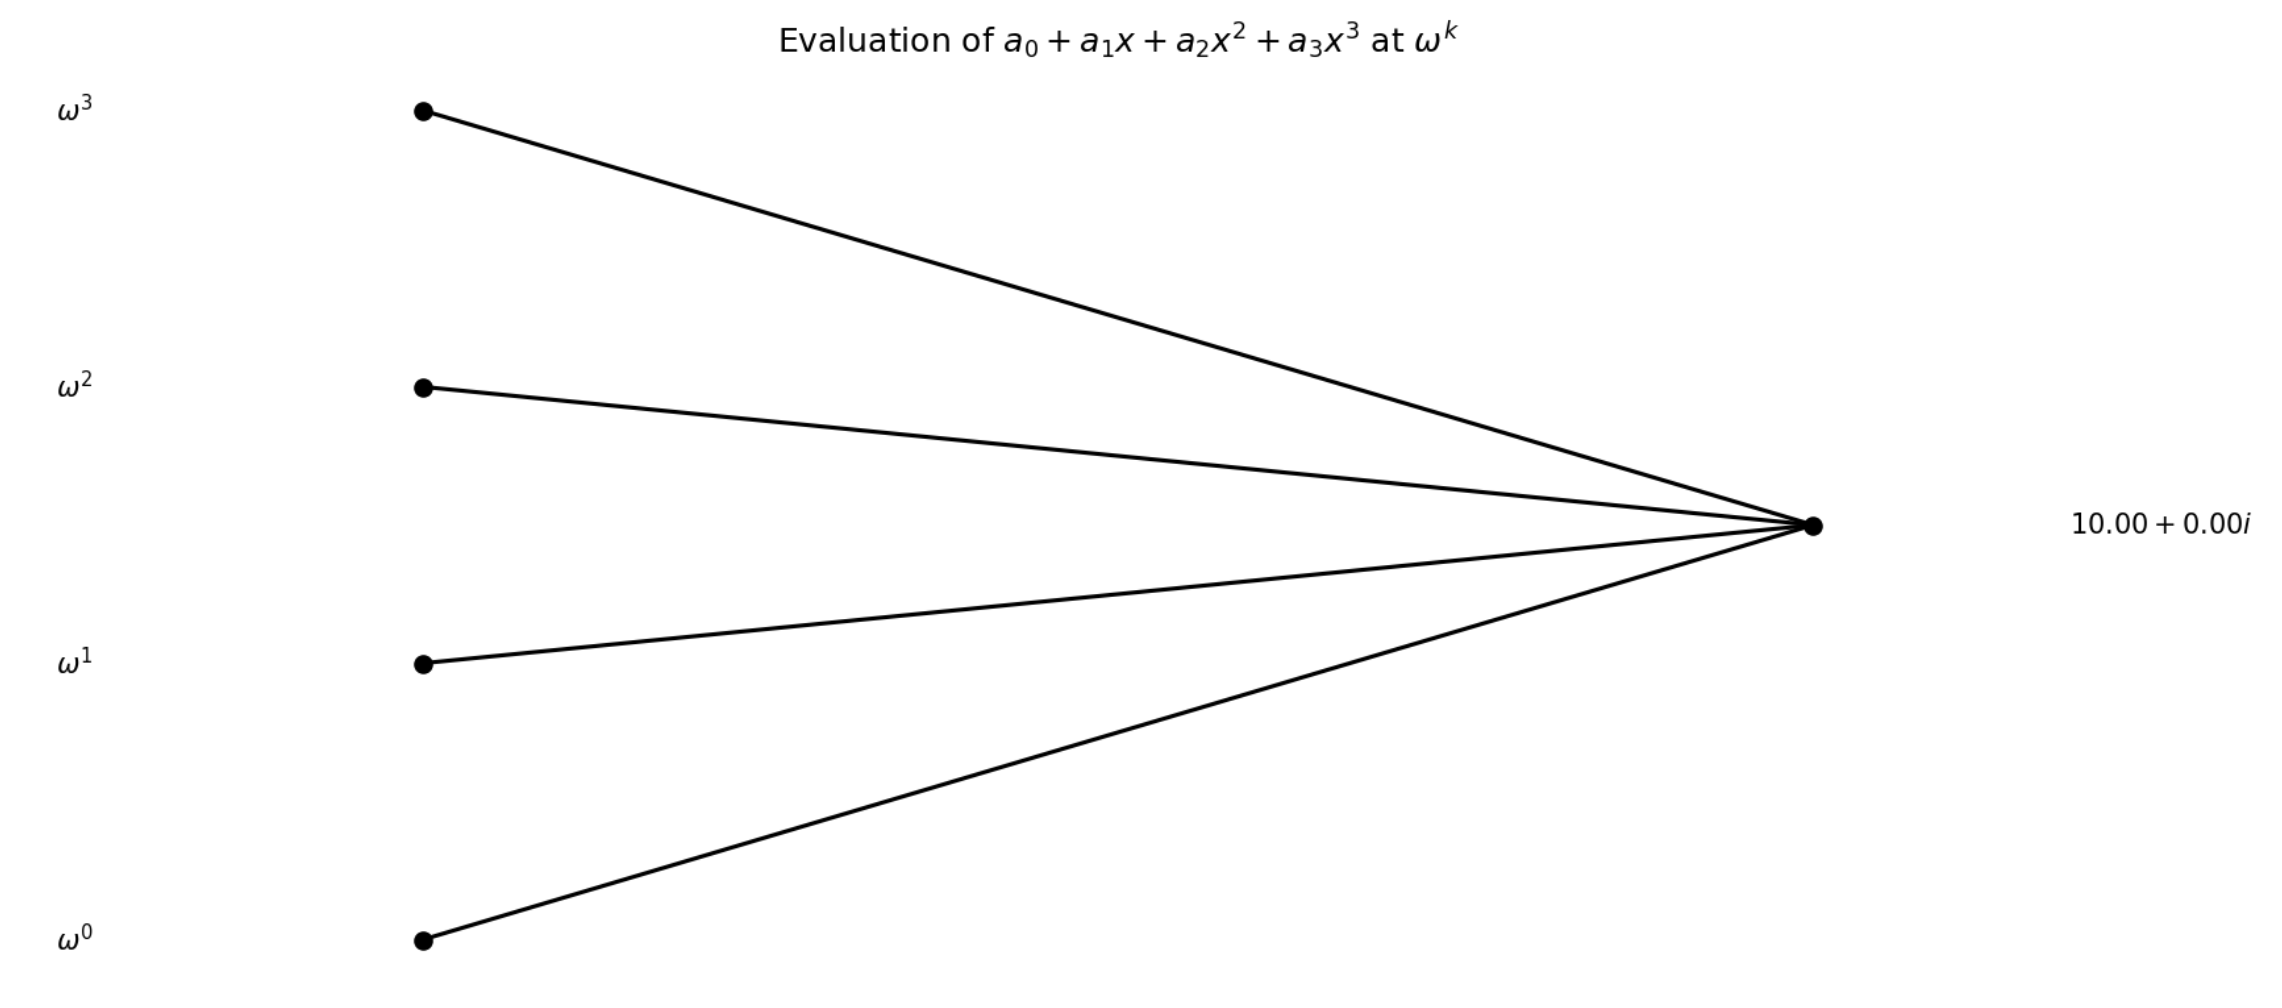
\includegraphics[width=0.75\linewidth]{Screenshot 2024-04-09 at 16.08.00.png}
    \caption{Final result using FFT}
\end{figure}

\section{Question 2}
The algorithm privided is wrong because:

The FFT can indeed be used for efficient polynomial multiplication by performing the following steps:

\begin{enumerate}
    \item Evaluate each polynomial at the \( n \) distinct powers of the primitive \( n^\text{th} \) root of unity.
    \item Multiply the corresponding values.
    \item Interpolate the product polynomial from these values.
\end{enumerate}

This works because polynomial multiplication in the coefficient space translates to pointwise multiplication in the value (or Fourier) space.

However, polynomial division is not as straightforward. Here's why the proposed algorithm doesn't work:

\begin{enumerate}
    \item \textbf{Evaluation:} While you can evaluate \( P(x) \) and \( Q(x) \) at the \( n \) powers of the primitive \( n^\text{th} \) root of unity, the evaluation itself is not an issue.
    \item \textbf{Pointwise Division:} The operation \( \frac{P(\omega^i)}{Q(\omega^i)} \) assumes that \( Q(\omega^i) \neq 0 \) for all \( i \). If \( Q(x) \) has any roots that are also \( n^\text{th} \) roots of unity (which is entirely possible), the division by \( Q(\omega^i) \) will be undefined at those points.
    \item \textbf{Interpolation:} Even if \( Q(\omega^i) \) is non-zero for all \( i \), and you can compute \( \frac{P(\omega^i)}{Q(\omega^i)} \), interpolating these values to get the quotient polynomial only works if the division results in a polynomial, which is only the case when \( P(x) \) is divisible by \( Q(x) \) without remainder. In general, polynomial division results in a quotient and a remainder.
    \item \textbf{Polynomial Degree:} If \( P(x) \) and \( Q(x) \) are of different degrees, and \( P(x) \) is of higher degree, the resulting values after pointwise division will not correspond to the coefficients of a polynomial of degree less than or equal to \( n-1 \), which is necessary for a unique interpolation result.
\end{enumerate}

Therefore, the algorithm fails because it does not handle the case where \( Q(x) \) has roots that are \( n^\text{th} \) roots of unity and because it does not account for the possibility of a remainder. Also, the interpolation from value space to coefficient space is not guaranteed to yield a polynomial of degree \( n-1 \) or less.

For these reasons, this algorithm is not correct for polynomial division. The correct approach to polynomial division is more involved and cannot be simplified to an application of the FFT in the same manner as polynomial multiplication.
\section{Question 3}
We can utilize divide and conquer in this problem:

\subsection*{Algorithm Outline}
\begin{enumerate}
    \item \textbf{Distribution of Work}: Assign to each processor \( P_i \) two indices from vectors \( A \) and \( B \), such that \( P_i \) holds \( a_i \) and \( b_i \).
    \item \textbf{Local Computations}: Each processor \( P_i \) computes two sums locally:
    \begin{itemize}
        \item The first sum \( S1_i \) for \( c_i \) involves summing products \( a_j b_{i-j} \) for \( j = 0 \) to \( i \).
        \item The second sum \( S2_i \) for \( c_i \) involves summing products \( a_j b_{n+i-j} \) for \( j = i+1 \) to \( n-1 \), taking care to wrap the index of \( b \) around modulo \( n \).
    \end{itemize}
    \item \textbf{Parallel Prefix Sum}: Use a parallel prefix sum algorithm to compute the prefix sums for \( S1 \) and \( S2 \) in \( O(\log n) \) time.
    \item \textbf{Combine Results}: Each processor \( P_i \) then adds its two sums \( S1_i \) and \( S2_i \) to produce \( c_i \).
    \item \textbf{Communication}: Communicate the results to form the final vector \( C \), if necessary.
\end{enumerate}

\subsection*{Pseudocode}
\begin{verbatim}
procedure compute_positive_wrapped_convolution(A, B, n):
    // Step 1: Distribution of Work
    parallel for i = 0 to n-1 do:
        P_i holds a_i and b_i

    // Step 2: Local Computations
    parallel for i = 0 to n-1 do:
        S1_i = sum(a_j * b_{i-j} for j = 0 to i)
        S2_i = sum(a_j * b_{(n+i-j) mod n} for j = i+1 to n-1)

    // Step 3: Parallel Prefix Sum
    S1 = parallel_prefix_sum(S1, n)
    S2 = parallel_prefix_sum(S2, n)

    // Step 4: Combine Results
    parallel for i = 0 to n-1 do:
        c_i = S1_i + S2_i

    // Step 5: Communication
    // (Depends on the model of parallel computation used)

    return C = (c_0, c_1, ..., c_{n-1})
end procedure
\end{verbatim}

\subsection*{Complexity}
\begin{itemize}
    \item The \textbf{Parallel Prefix Sum} operation is a key component of the algorithm that computes all prefix sums of an input sequence in \( O(\log n) \) time using \( n \) processors.
    \item \textbf{Wrap-Around Indexing}: The term \( b_{n+i-j} \) for \( j > i \) corresponds to \( b_{i-j} \) when the indexing is modulo \( n \).
    \item The \textbf{Time Complexity} of the algorithm is \( O(\log n) \), with the parallel prefix sum being the most time-consuming operation.
\end{itemize}

\section{Question 4}
A matrix is called Toeplitz if all the entries along each diagonal of the matrix are equal. We can easily write a Toeplitz matrix if its first row and first column are given. Thus, an \( n \times n \) Toeplitz matrix has only \( 2n-1 \) distinct elements.
\[
\begin{aligned}
& \text{row vector} = \begin{bmatrix}
t_{n-1} & t_{n-2} & \cdots & t_1 & t_0
\end{bmatrix} = r \text{ (say).} \\
& T_n = \operatorname{Toep}\begin{bmatrix}
t_{n-1} & t_{n-2} & \cdots & t_1 & t_0 \\
t_{n} & t_{n-1} & \cdots & t_2 & t_1 \\
\vdots & \vdots & \ddots & \vdots & \vdots \\
t_{2n-2} & t_{2n-3} & \cdots & t_{n} & t_{n-1}
\end{bmatrix}
\end{aligned}
\]

Given a Toeplitz matrix \( T_n \) and a vector of length \( n \); to compute their product, we embed it in the product of a Circulant matrix of order \( 2n \) of the given form
\[
C_{2n} = \begin{bmatrix}
T_n & U_n \\
U_n & T_n
\end{bmatrix}
\]
with a vector of length \( 2n \) whose first \( n \) elements are the same as the elements of the given vector, and the next \( n \) elements are all zeros. Thus,
\[
\begin{aligned}
& C_{2n} \cdot \begin{bmatrix}
V_{n \times 1} \\
O_{n \times 1}
\end{bmatrix} = \begin{bmatrix}
T_n & U_n \\
U_n & T_n
\end{bmatrix} \begin{bmatrix}
V_{n \times 1} \\
O_{n \times 1}
\end{bmatrix} \\
& = \begin{bmatrix}
T_n V_{n \times 1} \\
U_n V_{n \times 1}
\end{bmatrix}
\end{aligned}
\]

Our desired answer is \( T_n V_{n \times 1} \), where \( V_{n \times 1} = \begin{bmatrix}
a_0 & a_1 & \cdots & a_{n-1}
\end{bmatrix}^T \).
So, given a Toeplitz matrix of order \( n \times n \) and a vector of length \( n \), we first write the Circulant matrix of order \( 2n \times 2n \) using the given Toeplitz matrix and the vector \( \begin{bmatrix}
\text{given vector} \\
O_{n \times 1}
\end{bmatrix} \xrightarrow{\text{(as \( I_n \) column)}} = V_{2n \times 1} \) (say). Then we compute \( C_{2n} \cdot V_{2n \times 1} \) using FFT in four steps. From this product, we can extract our desired result -- the product of \( T_n \) and the given vector.
\section{Question 5}

\begin{enumerate}
    \item Assume we have an input array \( A \) of \( n \) distinct elements and \( n^2 \) processors. We also have a temporary array \( T \) of size \( n \), initialized to 0.
    
    \item Each processor \( P_{ij} \) is assigned to a pair of elements \( (A[i], A[j]) \), where \( 0 \leq i, j < n \).
    
    \item Each processor \( P_{ij} \) reads its corresponding elements and performs the following:
    \begin{itemize}
        \item If \( A[i] > A[j] \), processor \( P_{ij} \) writes a 1 into \( T[i] \).
        \item Otherwise, \( P_{ij} \) does nothing.
    \end{itemize}
    
    \item After all processors have done this, the array \( T \) will contain the number of elements that are smaller than \( A[i] \) for each \( i \), because the writes are summed up in the case of concurrent writes.
    
    \item Finally, write \( A[i] \) to the output array \( B \) at the index \( T[i] \), which gives us the sorted array \( B \).
\end{enumerate}

\subsection*{C++ Code Simulation}
The C++ realization can be as follows:

\begin{lstlisting}
#include <iostream>
#include <vector>
#include <thread>
#include <mutex>

std::mutex write_mutex; // Mutex for simulated concurrent writing

// Simulated concurrent write operation
void concurrent_write(std::vector<int>& arr, int index) {
    std::lock_guard<std::mutex> guard(write_mutex);
    arr[index]++; // Protected by mutex to simulate summing concurrent writes
}

void parallel_sort(const std::vector<int>& input, std::vector<int>& sorted) {
    const int n = input.size();
    std::vector<int> T(n, 0);
    std::vector<std::thread> threads;

    // Create n^2 threads to compare each pair of elements
    for (int i = 0; i < n; ++i) {
        for (int j = 0; j < n; ++j) {
            threads.emplace_back([&input, &T, i, j]() {
                if (input[i] > input[j]) {
                    concurrent_write(T, i);
                }
            });
        }
    }

    // Wait for all threads to complete
    for (auto& thread : threads) {
        thread.join();
    }

    // Place the elements into their sorted position
    for (int i = 0; i < n; ++i) {
        sorted[T[i]] = input[i];
    }
}

int main() {
    std::vector<int> input = {3, 1, 4, 1, 5, 9, 2, 6, 5};
    std::vector<int> sorted(input.size(), 0);

    parallel_sort(input, sorted);

    for (int num : sorted) {
        std::cout << num << " ";
    }
    std::cout << std::endl;

    return 0;
}
\end{lstlisting}

\textbf{The above algorithm runs in \( O(1) \) time because all operations are done in parallel by \( n^2 \) processors.} Each processor performs a single comparison and possibly a single write, both of which are constant time operations.

However, this algo is of 0 practical value because the algorithm requires \( n^2 \) processors for \( n \) elements, which is impractical for large \( n \) due to hardware limitations and cost. Also The number of processors required grows quadratically with the number of input elements, making it unscalable. The CRCW PRAM Sum Model is a theoretical abstraction and concurrent writes with summation are not typically supported by real hardware. Even if we had the required number of processors, the overhead of managing them and coordinating the writes would outweigh the benefits of the \( O(1) \) running time.


\end{document}